\documentclass[../../main.tex]{subfiles}

Im Folgenden Text betrachten wir meine Konzepte bezüglich Videospielen in einer Kinderklinik und deren Übertrag in die Architektur. Da die Umfrageauswertung ausschlaggebende Informationen zu den Bedürfnissen potentieller Patienten gibt, stelle ich meine Ideen auch im Bezug dieser dar. Im Gegensatz zum Thema der Gerätegestaltung gibt es hier keine große Gefahr, Kinder mit einem unangenehmen Design abzuschrecken; trotzdem ist es wichtig, den Patientenaufenthalt auch durch die visuelle Gestaltung der Spielegeräte im Rahmen meiner Möglichkeiten angenehm zu machen.

So habe ich z. B. ein Konsolendesign konzipiert, welches zum Raumdesign der Klinik passt und nicht zu sehr heraussticht (Abb. \ref{fig:konsolendesign}).
\begin{figure}[ht]
    \centering
    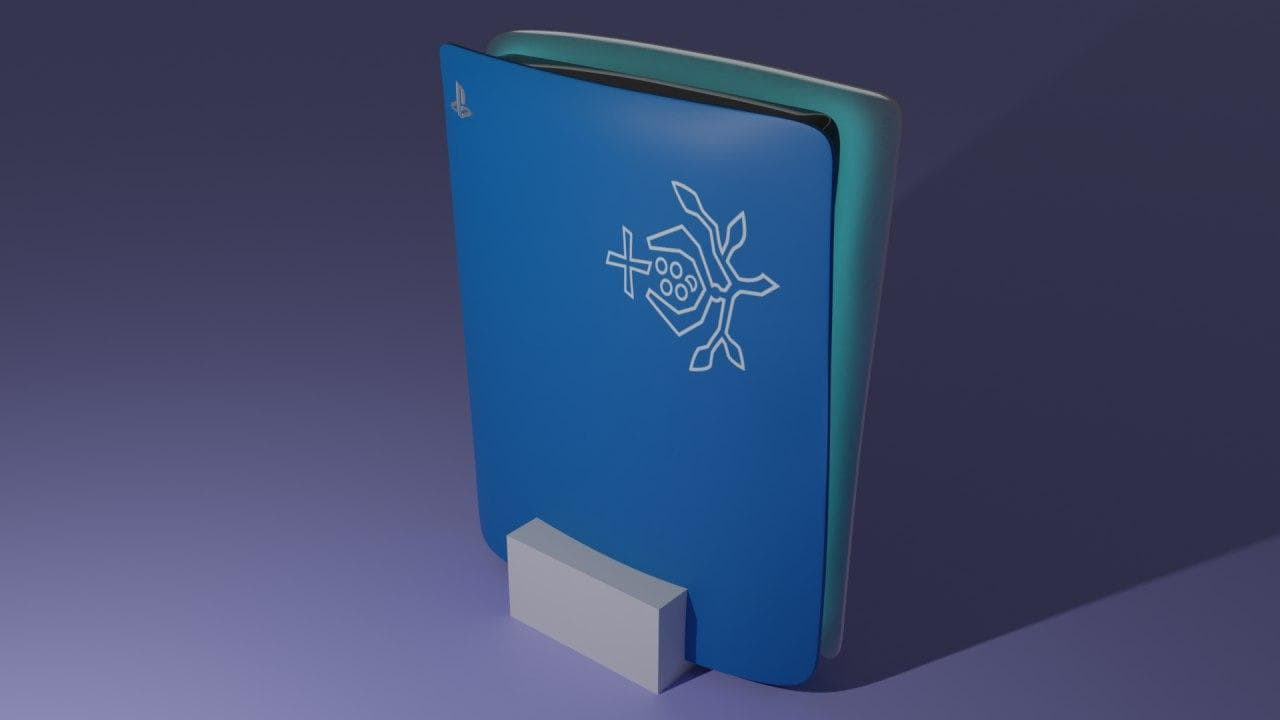
\includegraphics[width=\textwidth]{ps5_branded.jpg}
    \caption{PS5 mit Logo der Barmherzigen Brüder. \footnotesize{(``Sony PlayStation 5'' by Spellmansp is licensed under Creative Commons Attribution. https://skfb.ly/6UtSN To view a copy of this license, visit http://creativecommons.org/licenses/by/4.0/.)}}
    \label{fig:konsolendesign}
\end{figure}
Gegen den Einsatz eines solchen Designs spricht jedoch, dass es mit Sicherheit dem Patienten Fremd sein würde und kein Gefühl von Familiarität erwecken würde.

Ein wichtigerer und weniger ambiguöser Teil ist das Verstecken von Kabeln. In einem Patientenzimmer gibt es oft schon genügend gruselige Maschinen und Kabel - das muss beim Gaming-System nicht sein. Gutes Kabel-Management ist also gerade hier notwendig für ein positives visuelles Bild der Geräte. Führen wir alle Kabel zwischen Fernseher und Konsole zusammen, ist das Problem schon gelöst (Abb. \ref{fig:cable_management}). Darüber hinaus verwenden wir natürlich drahtlose Controller - eine Substantielle Verzögerung ist nicht Vorhanden.
\begin{figure}[ht]
    \centering
    \includegraphics[width=0.8\textwidth]{example-image} % TODO Bild cable management
    \caption{Kabelmanagement}
    \label{fig:cable_management}
\end{figure}

Da die förderung von selbstgebrachten Konsolen laut Umfrageergebnissen durchaus erwünscht ist, musste ich mir auch hierzu etwas einfallen lassen. Weil die Nintendo Switch, Smartphones und Laptops zu den bedeutendsten tragbaren Konsolen gehören, maßschneidere ich meine Ideen vor Allem auf diese. Für alle drei wäre es grundlegend wichtig, eine Möglichkeit zum Aufladen anzubieten.